\documentclass[12pt,a4paper]{article}
\usepackage[latin1]{inputenc}
\usepackage{amsmath}
\usepackage{amsfonts}
\usepackage{amssymb}
\usepackage{graphicx}
\usepackage{float}
\date{}
\author{Philipp Burt}
\title{Differentialgleichungen - ein kleiner Ueberblick}
\begin{document}
	\maketitle
	\tableofcontents
\section*{Vorbemerkungen}
Dieses Dokument soll als Hilfestellung zur Behandlung von Differentialgleichungen im Rahmen der Mathe II Vorlesung f�r Biologiestudierende dienen. Es erhebt weder Anspruch auf Vollstaendigkeit noch Richtigkeit. Zudem kann nicht davon ausgegangen werden, dass alle Themenbereiche der Klausur abgedeckt werden. 
\section{Was ist ueberhaupt eine Differentialgleichung?}
 Eine klassische Funktion die das Grundkonzept einer DGL verkoerpert ist die Exponentialfunktion. Deren Funktionenwert ist in jedem Punkt gleich dem Wert der Ableitung. Mathematisch laesst sich dies so ausdruecken:
\begin{eqnarray}
f(x)=e^{x} \rightarrow f'(x)=e^{x}=f(x)
\end{eqnarray}
Betrachten wir als naechstes folgende Funktion.
\begin{equation}\label{DGL 1}
x'(t)=a \cdot x(t)
\end{equation}
Diese Funktion besagt, dass die Ableitung der Funktion x an jeder Stelle gleich der Funktion selbst ist, multipliziert mit einem Faktor a. Wahrend die Exponentialfunktion immer genau ihrer Ableitung entspricht koennte man sich auch Beziehungen zwischen Funktionen und ihrer Ableitung vorstellen, die komplizierter sind. Oft ist es so, dass man das Verhaeltnis von Ableitung und Funktion kennt, aber die Loesungsfunktion selbst erst aus dieser Beziehung finden muss. Ob eine Funktion eine Differentialgleichung erfuellt laesst sich pruefen, indem man ihre Ableitung bildet und in die Gleichung einsetzt. Pruefen wir ob die Gleichung 
\begin{equation}\label{Lsg1}
x(t)=e^{a*t}
\end{equation}
Die Differentialgleichung \ref{DGL 1} erfuellt:
\begin{equation}
x(t)=e^{a*t} \rightarrow x'(t)=a \cdot e^{a*t}
\end{equation}
Da aber:
\begin{equation}
e^{a*t}=x(t) \rightarrow x'(t)=a \cdot x(t)
\end{equation}
Gleichung \ref{Lsg1} erfuellt also die Bedingungen unserer DGL \ref{DGL 1}. Das heisst aber noch nicht, dass es nicht auch noch andere Loesungen gibt, die diese Differentialgleichung erfuellen. Im allgemeinen ist es so, dass es mehrere Loesungen zu einer Differentialgleichung gibt. Erst bestimmte Anfangsbedingungen, eines Systems machen es moeglich, eine eindeutige Loesung zu berechnen. Mehr dazu in: allgemeine Loesung und Randbedingungen.
\newpage
\section{Wie klassifiziere ich eine Differentialgleichung?}
Differentialgleichungen koennen sehr unterschiedlich aussehen. Die meisten sind nicht so einfach zu loesen wie Gleichung \ref{DGL 1}. Es gibt jedoch Gleichungstypen, aus denen man auf Loesungsmoeglichkeiten schliessen kann. Dafuer bedarf es eines einheitlichen Vokabulars, wenn man ueber Differentialgleichungen spricht. Betrachten wir folgende Differentialgleichung: \\
\begin{equation}\label{DGL 2}
x'(t)=a(t) \cdot x(t)+b(t)
\end{equation}
Im Vergleich zu Gleichung \ref{DGL 1} faellt hier auf, dass der Term a zu a(t) geaendert wurde und zusaetzlich ein additiver Term b(t) an der Gleichung angefuegt wurde. Im allgemeinen benoetigen wir vier Kriterien zur Klassifikation von DGL:
\begin{enumerate}
	
	\item \textbf{Homogenitaet} \\
	
	Eine DGL ist homogen, wenn der additive Term b(t) fehlt. Also wenn nur Terme dastehen, die von x abhaengen.
	\item \textbf{Linearitaet}\\
	Eine DGL ist linear, wenn der Term x(t) \textbf{nur} in der ersten Potenz vorkommt. Das heisst eine DGL ist nicht linear in folgenden Faellen: es taucht gar kein Term x(t) auf, oder es kommen Terme wie $ x^{2}(t) $ oder $ x^{3}(t) $ oder auch $ \frac{1}{x(t)} $ vor (nicht linear!).
	
	\item \textbf{Ordnung} \\
	
	Die Ordnung einer Differentialgleichung bezieht sich immer auf den Ableitungsgrad. Die Ordnung entspricht dabei der h�chsten Ableitung, die in der Gleichung auftaucht.DGL \ref{DGL 1} und \ref{DGL 2} sind DGL erster Ordnung. Folgende Gleichung z.B. ist dritter Ordnung: \\
	\begin{equation}
	x'(t)=2 \cdot x'''(t)+5 \cdot x''(t)
	\end{equation}
	
	\item \textbf{Koeffizienten} \\
	
	Koeffizienten koennen entweder variabel oder konstant sein. Das ist in DGL \ref{DGL 2} durch das a(t) und b(t) angedeutet. Das heisst in diesem Fall koennten a und b abhaengig von t sein. Z.B. koennte DGL \ref{DGL 2} so aussehen: \\
	\begin{equation}
	x'(t)=t \cdot x(t)+t^{2}
	\end{equation}
	In diesem Fall sind sowohl a(t)=t und $ b(t)=t^{2} $ von t abhaengig. Es reicht aber schon wenn mindestens ein Koeffizient in der DGL von t abhaengt. Dann spricht man von variablen koeffizienten. Sind alle Koeffizienten konstant, spricht man von konstanten Koeffizienten: \\
	\begin{equation}
	x'(t)=a \cdot x(t)+b
	\end{equation}
\end{enumerate}
Beispiele:
\begin{eqnarray}
x'(t)=x''(t)+t \cdot x(t) \\
\end{eqnarray}
2. Ordnung, var. Koeffizienten, homogen, linear
\begin{equation}
0=x'(t)+x^{2}+5
\end{equation}
1. Ordnung, konst. Koeffizienten, inhomogen, nicht linear
\newpage
\section{Wie loese ich eine Differentialgleichung?}
	\subsection{Stabilitaetsanalyse}
	Eine der einfachsten Fragen, die man sich ueber eine DGL stellen kann ist die Folgende: Gibt es einen Punkt, an dem sich mein System nicht aendert?\\
	In diesem Fall muss die Aenderung mit der Zeit (die Ableitung!) gleich Null sein, also sind die \textbf{Fixpunkte} $ \mathbf{x^{*}} $ meines Systems die Punkte, fuer die die Ableitung gleich Null wird.\\
	Beispiel: \\
	\begin{equation}
	x'(t)=5x-10 \rightarrow x'(t)=0=5x^{*}-10 \rightarrow x^{*}=2
	\end{equation}
	Fuer den Anfangswert x=2 aendert sich das System nicht. \\
	Fixpunkte koennen stabil oder instabil sein. Ein stabiler Fixpunkt ist ein Punkt, bei dem kleine Auslenkungen ueber die Zeit nicht zu einer langfristigen Aenderung fuehren. Bei einem instabilen Fixpunkt wuerde sich das System bei einer kleinen Auslenkung vom Fixpunkt weg bewegen. Vorstellen kann man sich das anschaulich mit einer Kugel, die auf der Spitze eine Berges liegt. Stoesst man die Kugel an, rollt sie den Berg runter und nimmt nicht wieder den ursprungswert an. Liegt die Kugel stattdessen in einem Tal, rollt die Kugel nach kleinen Auslenkungen wieder an der Urpsrungsort zurueck (s. Fig. \ref{fig:stability_analysis_3}). \\
	\begin{figure}
\centering
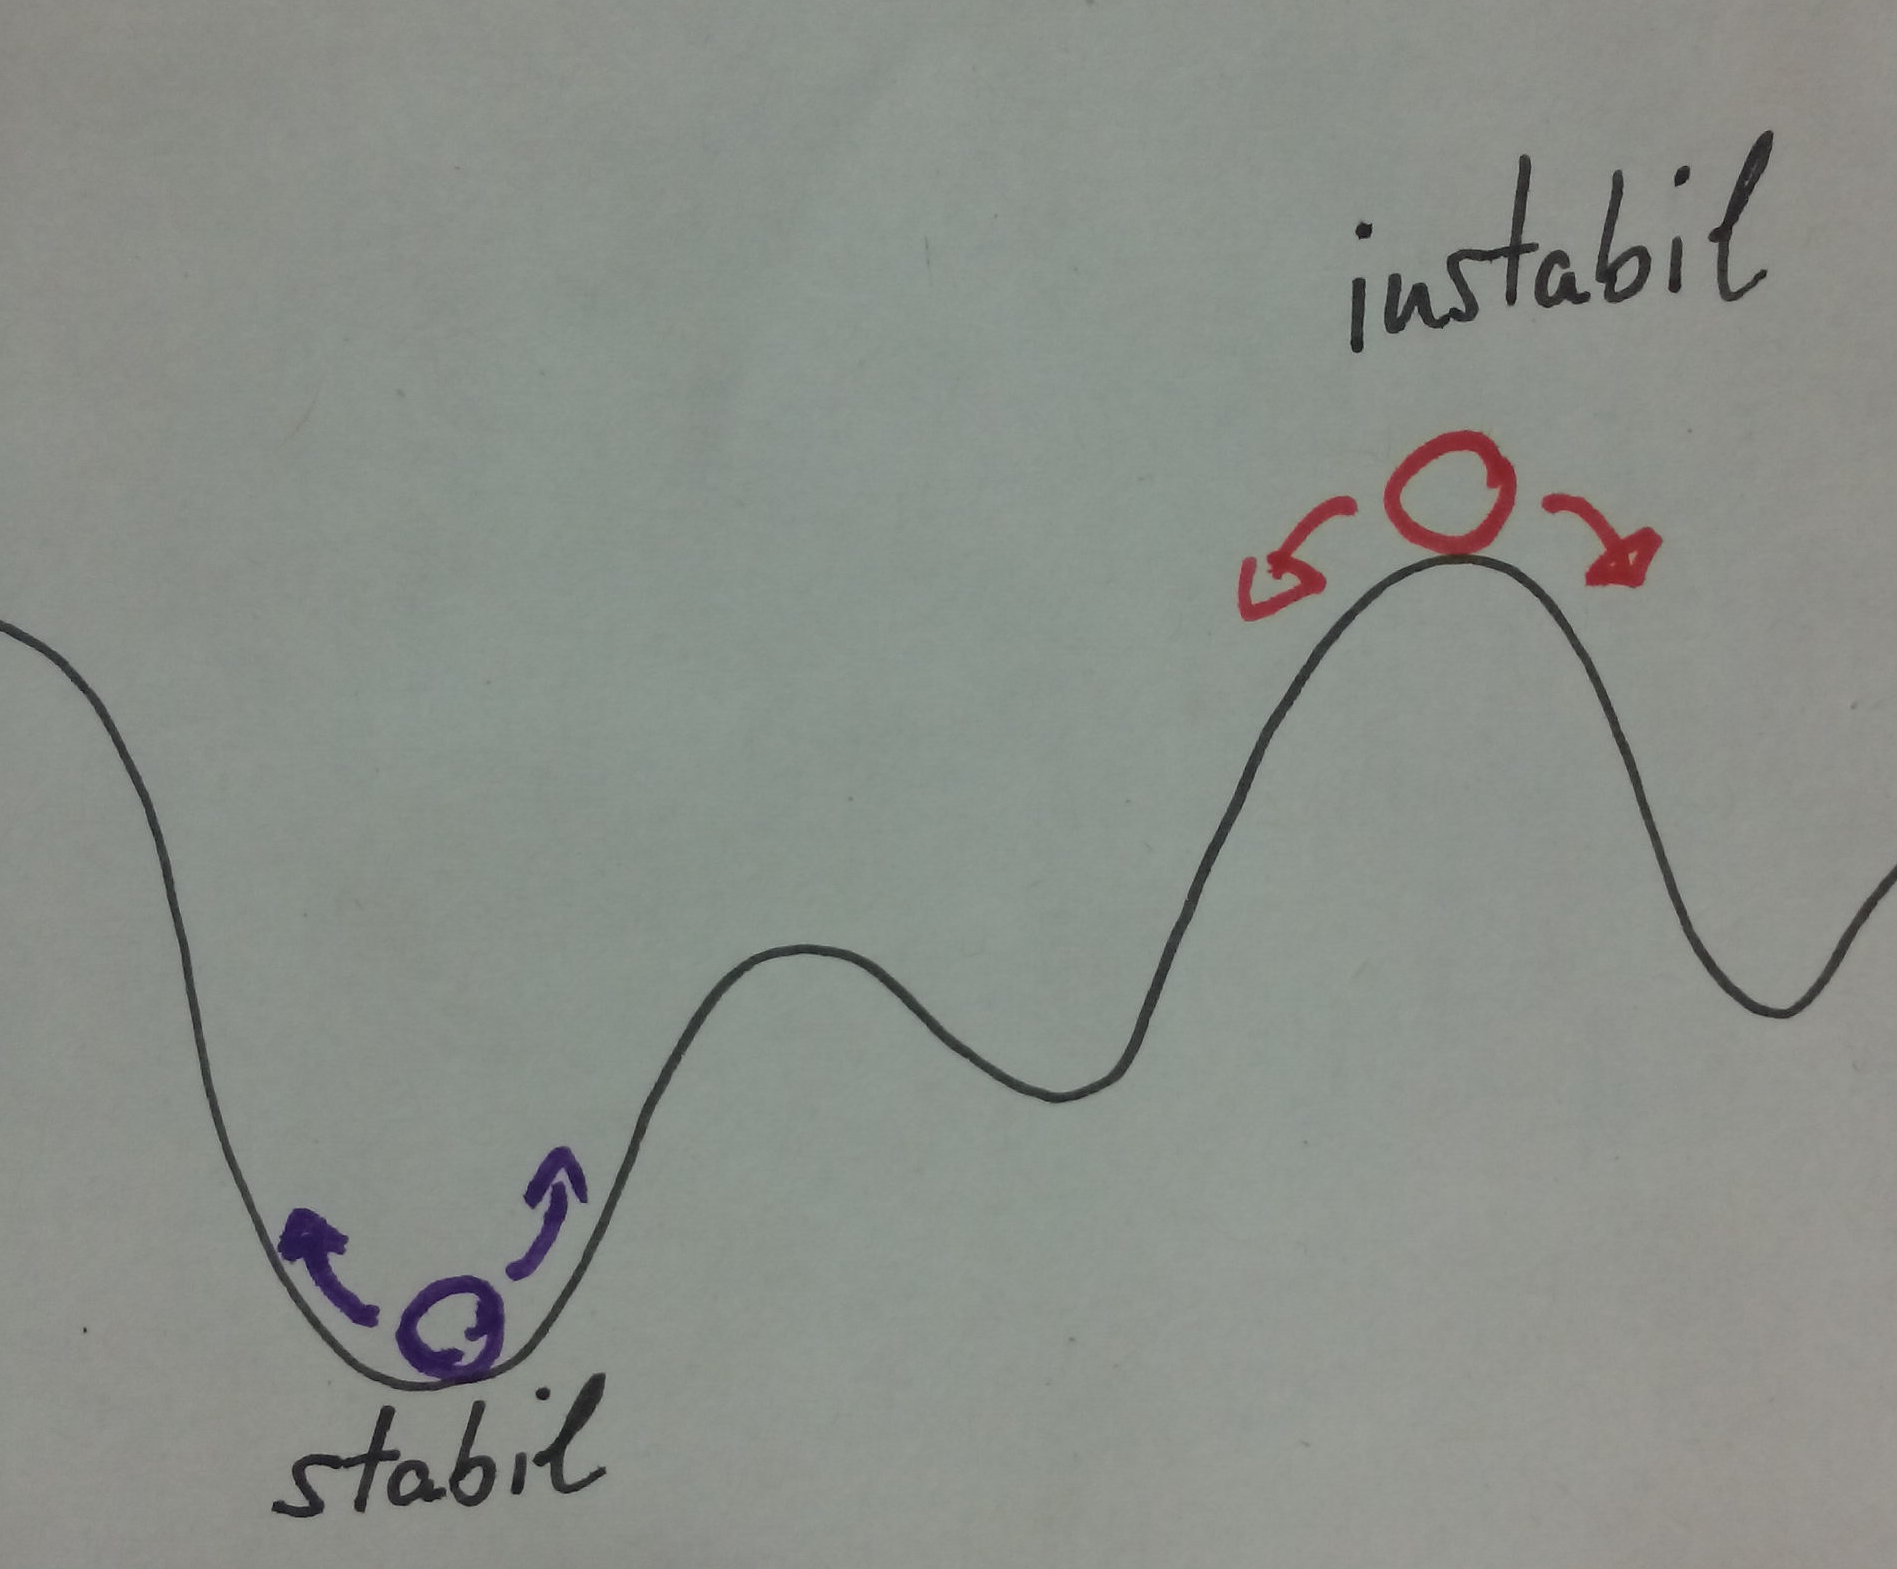
\includegraphics[width=0.7\linewidth]{stability_analysis_3}
\caption{Stabilitaet eines Balls in einer Berglandschaft als Beispiel fuer die Stabilitaet eines Systems, das durch Differentialgleichungen beschrieben wird.}
\label{fig:stability_analysis_3}
\end{figure}
	\subsection{Qualitative Loesung von Differentialgleichungen}
	Oft kann man durch qualitative Analyse und Berechnung der Fixpunkte viel ueber das Verhalten einer DGL aussagen. Die Fixpunkte sind die Nullstellen der Funktion f(x). Die Stabilitaet laesst sich anhand der Steiung ablesen. Betrachten wir eine beliebige DGL: \begin{equation}
		x'(t)=f(x)
	\end{equation}
	Die Fixpunkte $ x^{*} $ finden sich wenn man f(x) gleich Null setzt (s. Fig. \ref{fig:stability_analysis_1}).
\begin{figure}
\centering
\includegraphics[width=\linewidth]{stability_analysis_1}
\caption{Links: Die Fixpunkte sind die Nullstellen der Funktion f(x). Stabilitaet und langfristiges Verhalten der Loesung wird durch rote Pfeile angedeutet. Rechts: Die Loesungen x(t) wandern langfristig zu den stabilen Fixpunkten.}
\label{fig:stability_analysis_1}
\end{figure}
 Der Fixpunkt ist \textbf{stabil}, wenn $ f'(x^{*}) < 0 $ ist und \textbf{instabil}, wenn $ f'(x^{*}) > 0 $ ist. Kennt man die Fixpunkte und deren Stabilitaet kann man die Loesung graphisch darstellen, ohne sie genau zu kennen (s. Fig. \ref{fig:stability_analysis_1}
	\subsection{Quantitative Analyse von Differentialgleichungen}
	\subsubsection{Die allgemeine Loesung, Superposition und Randbedingungen}
	Wir haben schon gesehen, dass es fuer eine DGL mehrere Loesungen geben kann. Das Superpositionsprinzip besagt (fuer lineare DGL), dass jede Linearkombination zweier L�sungen auch wieder ein Loesung ergibt. Kennen wir also zwei Loesungen $ x_{1}(t) $ und $ x_{2}(t) $ koennen wir die allgemeine Loesung als Linearkombination schreiben: \begin{equation}\label{superposition}
	x(t)=a*x_{1}(t)+b*x_2{t}
	\end{equation} \\ In der Biologie beschreiben DGL zB. oft Wachstumsprozesse. Eine Loesung koennte dann das Wachstum einer Population beschreiben. Dabei spielt die Groesse der Anfangspopulation eine wichtige Rolle. Ist die Anfangspopulation Null kann offensichtlich auch kein Wachstum erfolgen. In diesem Fall ist die Groesse der Anfangspopulation die Anfangsbedingung. Abstrahiert man dieses Konzept kann man fuer jede Differentialgleichung die das Verhalten eines Systems beschreibt, bestimmte Bedingungen festlegen, die das System initialisieren. Betrachten wir nochmal Gleichung \ref{superposition}. Die allgemeine Loesung hat zwei unbekannte Parameter a und b. In diesem Fall braeuchte man zwei Anfangsbedingungen um a und b festlegen zu koennen. Siehe dazu auch Abschnitt \ref{sec_expansatz}.
	\subsubsection{Trennung der Variablen}
	Der Ansatz, Variablen zu trennen funktioniert gut fuer homogene Differentialgleichungen (auch wenn die Koeffizienten variabel sind!). Betrachte die DGL:
	\begin{equation}
	\dfrac{dx}{dt}=t*x
	\end{equation}
	In diesem Fall trennt man die Variablen t und x, so dass jede auf seiner Seite steht und integriert dann beide Seiten:
	\begin{eqnarray}
	\dfrac{dx}{dt}=t \cdot x~ | \cdot dt, /x \\
	\dfrac{1}{x}~dx=t~dt~|~Integriere \\
	\int \dfrac{1}{x}~dx= \int t ~ dt \\
	ln(x)=\frac{1}{2}t^{2}+c \\	
	x(t)=e^{\frac{1}{2}t^{2}+c}
	\end{eqnarray}
	Wichtig: Die Integrale koennen als bestimmtes Integral geloest werden, oder unbestimmt. In diesem Fall muss die Integrationskonstante c beruecksichtigt werden. Sie kann durch eine Anfangsbedingung geloest werden. Beispiel: x(0)=1
	\begin{equation}
	x(0)=e^{0+c}=e^{c}=1 \rightarrow c=0
	\end{equation}
	\subsubsection{Exponentialansatz}\label{sec_expansatz}
Im Prinzip wurde die DGL \ref{DGL 1} mit den Exponentialansatz geloest. Man verfahert immer nach dem selben Prinzip: Man nimmt eine allgemeine Exponentialfunktion als Loesung an. Dann leitet man diese Loesung ab und guckt, ob die Loesung tatsaechlich die Gleichung erfuellt. Generell bietet sich der Exponentialansatz  fuer homogene DGL mit konstanten Koeffizienten an. Vor allem fuer DGL hoeherer Ordnung ist es sehr praktisch, da man nur ableiten muss.\\
Beispiel:\\
Betrachte die Funktion 
\begin{equation}\label{expansatz}
x'(t)=x''(t)-2x(t)
\end{equation}
Ansatz: \begin{equation}
x(t)=e^{a \cdot t} \rightarrow x'(t)=a*e^{a*t} \rightarrow x''(t)=a^2 \cdot e^{a \cdot t}
\end{equation} 
Einsetzen in \ref{expansatz} liefert:
\begin{equation}
a \cdot e^{a \cdot t}=a^2 \cdot e^{a \cdot t}-2 \cdot e^{a \cdot t}
\end{equation}
Ausklammern:
\begin{equation}
a \cdot e^{a \cdot t}=(a^{2}-2) \cdot e^{a \cdot t}
\end{equation}
Es folgt:
\begin{equation}
a=a^{2}-2 \rightarrow 0=a^{2}-a-2 \\
\rightarrow a_{1,2}=1/2\pm \sqrt{((1/4) + 2)}
\end{equation}
\begin{equation}
\rightarrow a_{1,2}=1/2\pm 1.5 \rightarrow a_{1}=2,a_{2}=-1
\end{equation}
Da die Gleichung zwei Werte fuer a liefert, ist die allgemeine Loesung:
\begin{equation}
x(t)=b \cdot e^{2t}+c \cdot e^{-t})
\end{equation}
Die Werte b und c muessen aus den Anfangsbedingungen berechnet werden. Nehmen wir zB. die Bedingungen x(0)=0 und x'(0)=1. Dann folgt: 
\begin{eqnarray}
x(0)=b \cdot e^{0}+c \cdot e^{0}=b+c=0 \\
x'(t)=2b \cdot e^{2t}-c \cdot e^{-t} \\ \rightarrow x'(0)=2b-c=1
\end{eqnarray}
Man erhaelt also ein Gleichungssystem mit zwei Unbekannten:
\begin{eqnarray}
b+c=0 \\2b-c=1 \\ \rightarrow addiere~I+II \\ \rightarrow 3b=1 \rightarrow b=1/3, c=-1/3
\end{eqnarray}
Es folgt:
\begin{equation}
x(t)=1/3~e^{2t}-1/3~e^{-t}
\end{equation}
Eine letzte Anmerkung: Der Exponentialansatz funktioniert auch mit komplexen Zahlen, denkt daran: $ \sqrt{a}=i \pm \sqrt{\mathbb{R}(a)}~|a\in \mathbb{C}, a < 0 $
	\subsubsection{Variation der Konstanten}
	Die Variation der Konstanten wird bei inhomogenen DGL angewandt. Hierfuer sei auf das Skript verwiesen.
\end{document}